\chapter{Design}

\section{Overall System Design}

\subsection{Short description of the main parts of the system}
\textbf{Gas, Electricity and Water metering system}
\begin{itemize}
\item{User Interface}

\item{Graphs and Charts}
\item{Database control}
\end{itemize}
User Interface:
\begin{itemize}
\item{The user will be presented with an interface which has two text boxes for the username and password and a button to proceed once they have entered their login details. These details will be unique and should only be known by the user they pertain to.}
\item{Once logged in to the system, the user will be presented with a new interface in which they can load a database and access the different functionalities of the system such as inputting readings from the meters into the system to be stored in the database, viewing calculated averages and future prices and viewing consumption rates for the current month and any previous months in different formats and graphs/charts.}
\item{The user will be able to navigate the different tabs of the interface via keyboard input or through tab buttons on a toolbar on the system}
\end{itemize}

Graphs and Charts:
\begin{itemize}
\item{There will be several Graphs and charts on the system such as Pie Charts, Bar Charts, Line Graphs, Scatter Diagrams, tables etc. This is beneficial because it means that the user has a range of visual representations to choose from and can therefore choose the one they like the most or can understand and interpret the easiest. Each type of chart will have their own individual option on the main interface.}
\item{There will be 3 of each type of chart/graph for Gas, Electricity and Water Consumption, with each set of charts/graphs on their own layouts which can be switched between from the menu bar or the tool bar.}
\end{itemize}

Database control:
\begin{itemize}
\item{On the menu bar and toolbar there will be options to open to close a database, format the database  or create a new one along with options to add or remove items from the database each with icons to represent them for ease of access}
\item{In addition to these buttons, there will be added functionality for keyboard shortcuts to make using the system as quick as possible}
\item{If the user chooses to add data then they will be taken to an interface which asks what table the data is for and if relevant, which consumption type it refers to and then the system will take the user to a new interface in which they can input the data they wish to add and submit it to the database.}
\item{If the user chooses to remove data from the database, they will be taken to a similar interface to the one for the input interface and will be asked to specify what this data pertains to and then provide a date and consumption type if relevent.}
\item{If the user chooses to format the database then they will be taken to a new interface which asks them if they are sure that they want to format the database and will have two buttons for confirmation}
\item{If the user chooses to create a new database, they will be taken to another interface where they will be prompted to input a name for the new database and the interface will also contain a button which when pressed prompts the user to find the location on their computer to store the new database}
\end{itemize}

\subsection{System flowcharts showing an overview of the complete system}

\section{User Interface Designs}
\begin{landscape}
\begin{figure}[H]
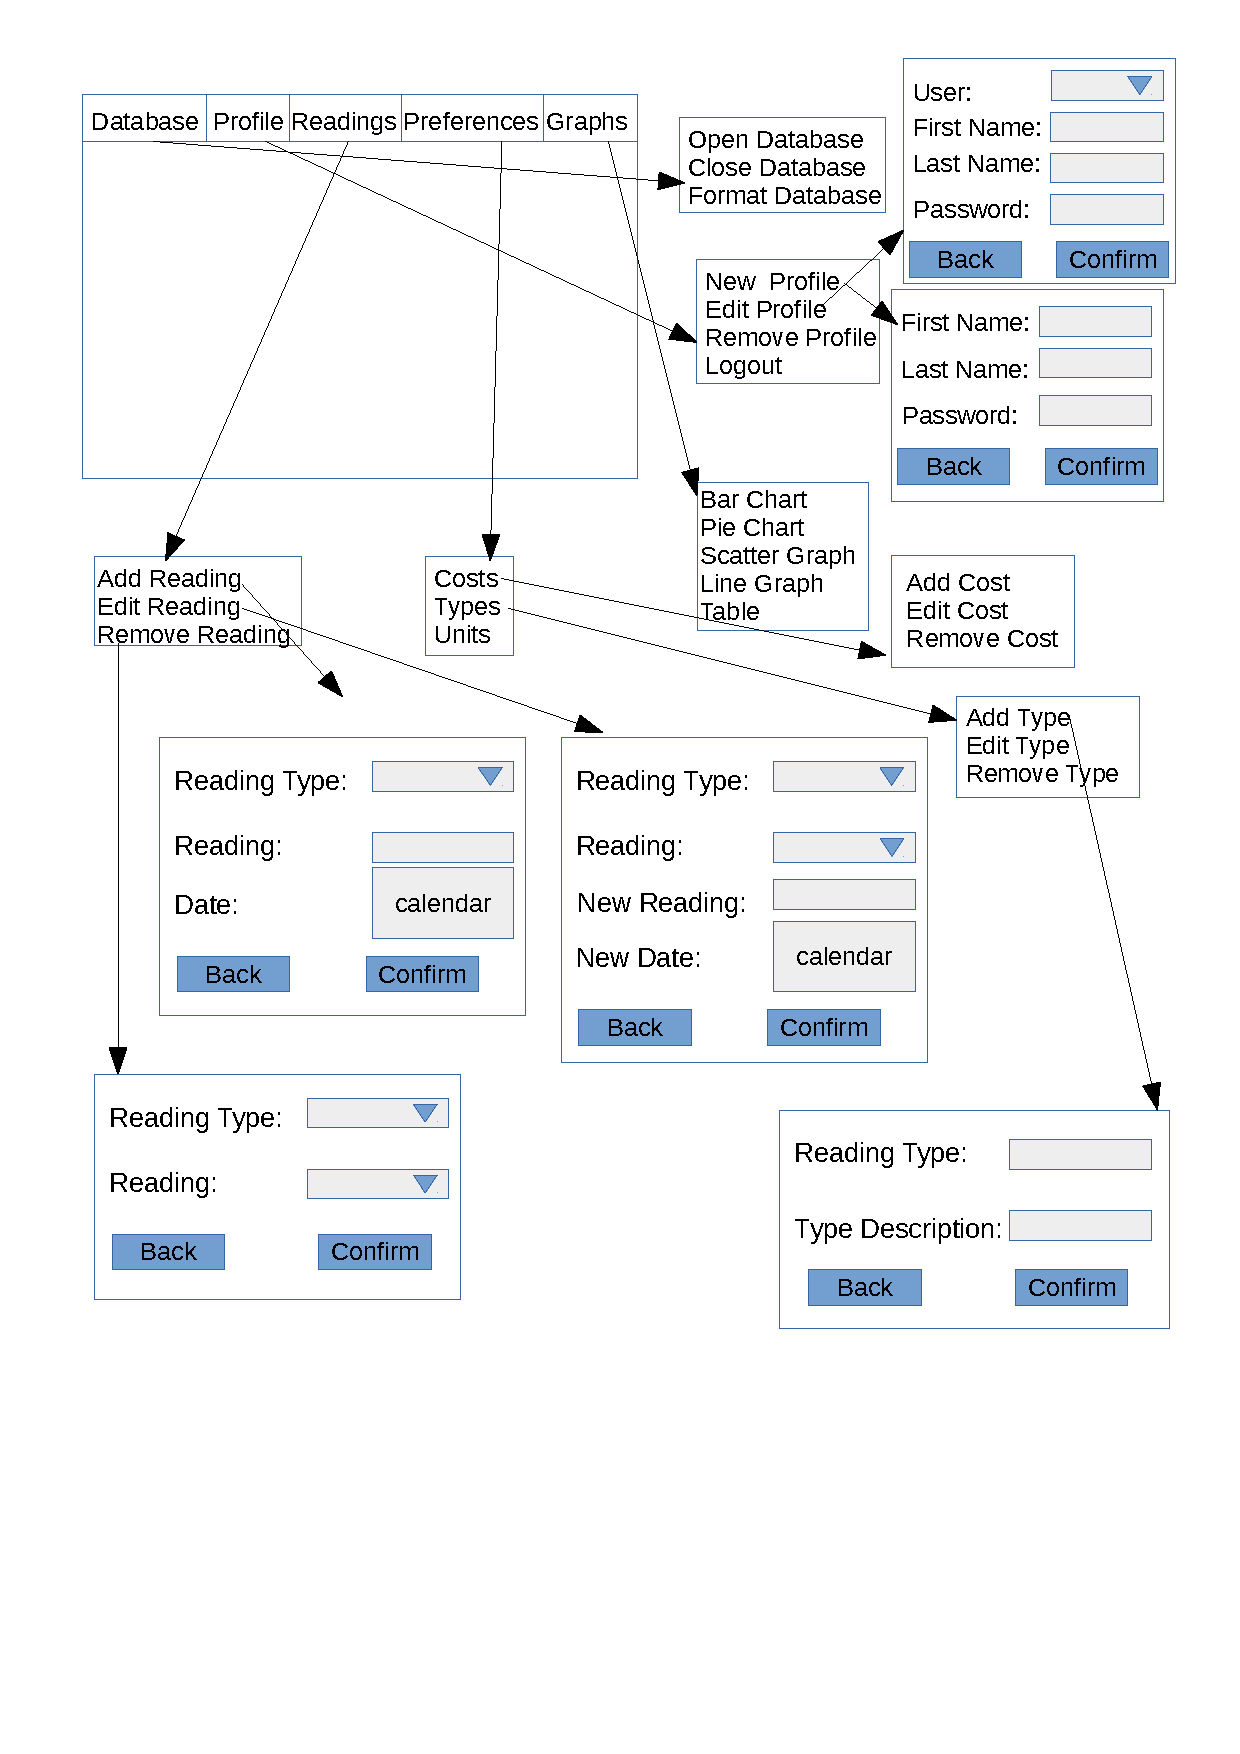
\includegraphics{./design/User Interface Design.pdf}
\caption{User Interface Design}
\end{figure}
\end{landscape}

\section{Hardware Specification}
The system will need to run on a laptop with a 1366x768 resolution screen with a 16:9  aspect ratio and running Windows 8. This is significant because it means I need to make sure the program will fit to this screen. A mouse will be required to navigate the program and select any inputs from drop down menus and a keyboard will be required to input data into text boxes on the program. The database for the program will be stored on a 1tb internal hard drive. In addition to that, the program can't be too intensive as the laptop only has a 1.5 ghz intel celeron dual core processor.
\section{Program Structure}

\subsection{Top-down design structure charts}
\begin{landscape}
\begin{figure}[H]
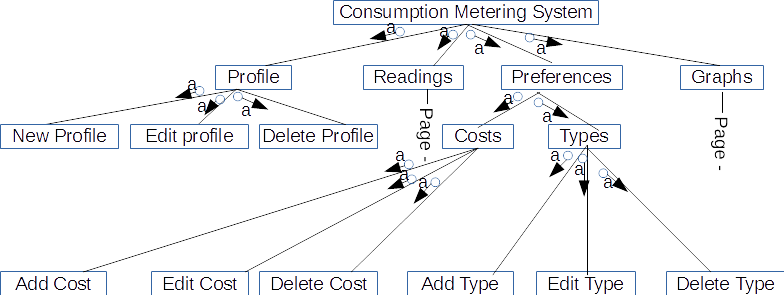
\includegraphics{./design/structure chart 1.png}
\caption{Top Down Structure Chart}
\end{figure}
\end{landscape}

\begin{landscape}
\begin{figure}[H]
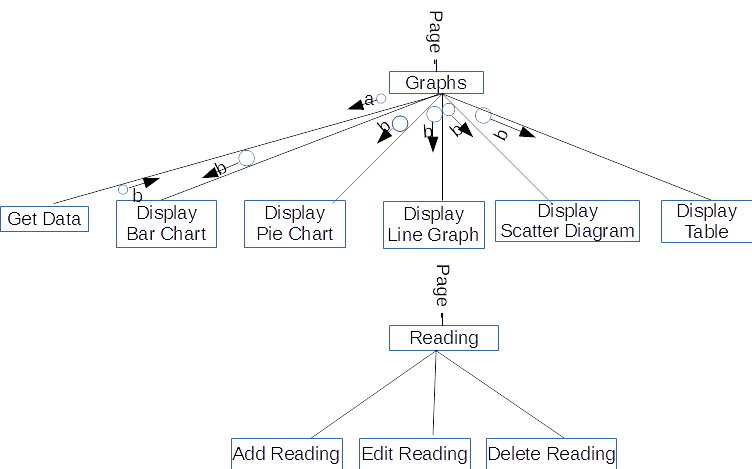
\includegraphics{./design/structure chart 2.png}
\caption {Top Down Structure chart}
\end{figure}
\end{landscape}

\begin{landscape}
\begin{figure}[H]
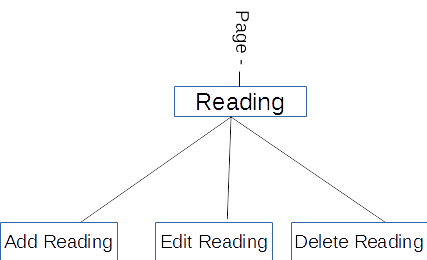
\includegraphics{./design/structure chart 3.png}
\caption{Top Down Structure Chart}
\end{figure}
\end{landscape}

\subsection{Algorithms in pseudo-code for each data transformation process}
\begin{algorithm}[H]
\label{fig:Calculate Average Consumption Cost}
\caption{Calculate Average Consumption Cost}
\begin{algorithmic}[1]
\Function{AverageConsumptionPrice}{ConsumptionPriceList,ConsumptionPrice}
\SET{$Total$}{$0$} 
\For{$ConsumptionPrice$}{$ConsumptionPriceList$}
\SET{$Total$}{$Total+ConsumptionPrice$}
\EndFor
\SET{$Average$}{$Total/Length_of_ConsumptionPriceList$}
\Return{$Average$}
\EndFunction
\end{algorithmic}
\end{algorithm}

\begin{algorithm}[H]
\label{fig:Calculate Average Consumption}
\caption{Calculate Average Consumption}
\begin{algorithmic}[1]
\Function{AverageConsumption}{ConsumptionList}
\SET{$Total$}{$0$}
\For{$Consumption$}{$ConsumptionList$}
\SET{$Total$}{$Total+Consumption$}
\EndFor
\SET{$Average$}{$Total/Length_of_ConsumptionList$}
\Return{$Average$}
\EndFunction
\end{algorithmic}
\end{algorithm}

\begin{algorithm}[H]
\label{fig:Convert Units}
\caption{Convert Units}
\begin{algorithmic}[1]
\Function{ConvertConsumptionUnits}{NewUnit,Consumption,CorrectionFactor,CalorificValue}
\If{$NewUnit = "Kilowatt Hours"$}
\SET{$NewConsumption$}{$(Consumption*CorrectionFactor*CalorificValue)/3.6$}
\Else
\SET{$NewConsumption$}{$(Consumption*3.6)/CorrectionFactor/CalorificValue$}
\EndIf
\Return{$NewConsumption$}
\EndFunction
\end{algorithmic}
\end{algorithm}

\subsection{Object Diagrams}
\begin{figure}[H]
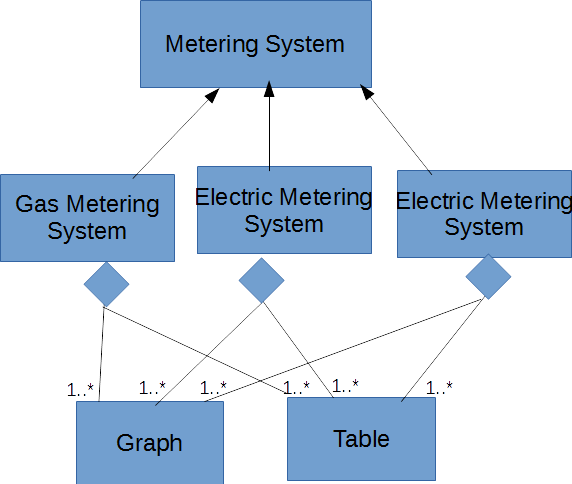
\includegraphics{./design/object diagram.png}
\caption{Object Diagram}
\end{figure}

\subsection{Class Definitions}
\begin{figure}[H]
\includegraphics{./design/userclassdefinitions.png}
\caption{User add,edit and remove class definitions}
\end{figure}

\begin{figure}[H]
\includegraphics{./design/typeclassdefinitions.png}
\caption{Type add,edit and remove class definitions}
\end{figure}

\begin{figure}[H]
\includegraphics{./design/costclassdefinitions.png}
\caption{Cost add,edit and remove class definitions}
\end{figure}

\begin{figure}[H]
\includegraphics{./design/readingclassdefinitions.png}
\caption{Reading add,edit and remove class definitions}
\end{figure}

\section{Prototyping}
I am going to prototype a tabbed interface as I would like to see if it is a suitable method to navigate between the different aspects of the system and to find out how to make one and display add the layers into the tabs.

I am also going to prototype graphs in Python as this is an integral part of the system and I need to know which graphs will be appropriate to use and how to make them and get them to display, I am also going to test to see which ones are appropriate to use for my system and which ones aren't suitable. This gives me a chance to make a more informed decision of which ones to use in the system.

\section{Definition of Data Requirements}

\subsection{Identification of all data input items}
\begin{itemize}
\item{UserID}
\item{First Name}
\item{Last Name}
\item{UserPassword}
\item{ReadingID}
\item{CostID}
\item{ReadingDate}
\item{CostPerUnit}
\item{CostStartDate}
\end{itemize}

\subsection{Identification of all data output items}
\begin{itemize}
\item{Average Consumption}
\item{Average Consumption Cost}
\item{Student User Name}
\item{Predicted Consumption}
\item{Predicted Consumption Cost}
\item{ConsumptionReading}
\item{ConsumptionType}
\item{ConsumptionTypeDescription}
\item{Consumption Cost}
\item{Consumption Reading Date}
\end{itemize}

\subsection{Explanation of how data output items are generated}
\begin{center}
\begin{tabular}{|p{5cm}|p{7.5cm}|}
	\hline
	\textbf{Output} & \textbf{How the output is generated} \\ \hline
	Average Consumption &  Calculated through AverageConsumption algorithm \\ \hline
	Average Consumption Cost & Calculated through AverageConsumptionPrice algorithm \\ \hline
	Student User Name & Generated from a combination of the user's first and last names \\ \hline
	Predicted Consumption & Calculated through PredictedConsumption algorithm \\ \hline
	Predicted Consumption Cost & Calculated through PredictedConsumptionCost algorithm \\ \hline
	ConsumptionReading & Fetched from database \\ \hline
	ConsumptionType & Fetched from database \\ \hline
	ConsumptionType Description & Fetched from database \\ \hline
	Consumption Cost & Calculated through ConsumptionCost algorithm \\ \hline
	Consumption Reading Date & Fetched from database \\ \hline
\end{tabular}
\end{center}

\subsection{Data Dictionary}
\begin{center}
\begin{tabular}{|p{4.3cm}|p{1cm}|p{1.5cm}|p{3cm}|p{1.5cm}|p{2.5cm}|}
	\hline
	\textbf{name} & \textbf{data type} & \textbf{length} & \textbf{validation} & \textbf{example data} & \textbf{comment} \\ \hline
	UserID & Integer & upto 4 digits & Unique number & 3141 & Holds unique ID for the user \\ \hline
	FirstName & String & 20 characters & upto 20 characters, not empty & John & Holds the user's first name \\ \hline
	LastName & String & 20 characters & upto 20 characters, not empty & Smith & Holds the user's last name \\ \hline
	UserPassword & String & 8-16 characters & Between 8 and 16 characters, contains a number and atleast one capital letter and/or special character & P@s\$w0rd & Holds the user's password \\ \hline
	ReadingID & Integer & upto 4 digits & Unique number & 5926 & Holds unique ID for the consumption reading \\ \hline
	ConsumptionReading & Float & upto 8 digits & Number upto 8 digits, not empty & 3.1415926 & Holds the reading for consumption \\ \hline
	ReadingDate & string & 8 characters & valid date, not empty & 05/12/14 & Holds the date of the reading \\ \hline
	ConsumptionType & String & Upto 11 characters & Is either Gas, Water or Electricity & Gas & Holds the consumption type \\ \hline
	ConsumptionTypeDescription & String & 50 characters & upto 50 characters, not empty & Monthly Gas Consumption & Holds a brief description of the consumption type \\ \hline
	CostID & integer & 4 Digits & Upto 4 digits & 2194 & Holds a unique ID for the cost \\ \hline
	CostPerUnit & float & 4 characters & Upto 4 characters & 2.14 & Holds a unit price for the consumption \\ \hline
	CostStartDate & string & 8 characters & Upto 8 characters & 04/12/2014 & Holds a date for the cost \\ \hline
\end{tabular}
\end{center}
\subsection{Identification of appropriate storage media}
As the system will only need to be accessed from one laptop, the database only needs to be stored onto that laptop. The data also needs to be accessed reasonably quickly so therefore it can be stored onto the internal hard drive. This also means it is easily accessed on the computer from any account and can also be stored on an external hard drive, online cloud storage or a memory stick for backups.
\section{Database Design}

\subsection{Normalisation}

\subsubsection{ER Diagrams}
\begin{figure}[H]
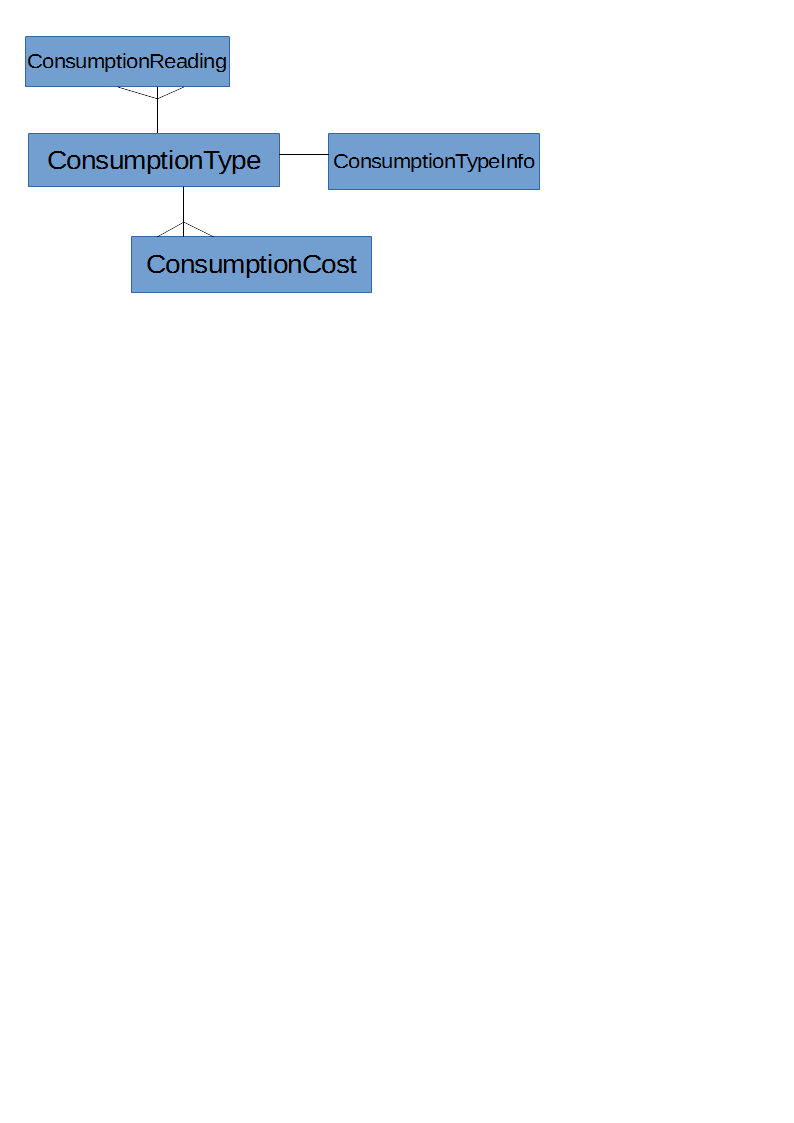
\includegraphics{./design/ER Diagrams.png}
\caption{ER Diagram}
\end{figure}

\subsubsection{Entity Descriptions}
Type(\underline{TypeID}, ConsumptionType,ConsumptionTypeDescription) \\
Reading(\underline{ReadingID},ConsumptionReading,ReadingDate,\emph{ConsumptionType}) \\
UserReading(\underline{UserReadingID},\emph{UserID},\emph{ReadingID}) \\
User(\underline{UserID},FirstName,LastName,UserPassword) \\
Cost(\underline{CostID},CostPerUnit,CostStartDate) \\
TypeCost(\underline{TypeCostID},\emph{CostID},\emph{ConsumptionType})\\

\subsubsection{1NF to 3NF}
\begin{center}
	\begin{tabular}{|p{5cm}|}
		\hline
		\textbf{UNF} \\ \hline
		UserID \\ \hline
		FirstName \\ \hline
		LastName \\ \hline
		UserPassword \\ \hline
		ReadingID \\ \hline
		ConsumptionReading \\ \hline
		ReadingDate \\ \hline
		ConsumptionType \\ \hline
		ConsumptionTypeDescription \\ \hline
		CostID \\ \hline
		CostPerUnit \\ \hline
		CostStartDate \\ \hline
	\end{tabular}
	
	\begin{tabular}{|p{5cm}|p{3.5cm}|}
		\hline
		\textbf{1NF} &  \\ \hline
		\textbf{Repeating} & \textbf{Non-repeating} \\ \hline
		\underline{ReadingID} \underline{UserID} & \underline{UserID} \\ \hline
		ReadingDate & FirstName \\ \hline
		ConsumptionReading & LastName\\ \hline
		ConsumptionType & UserPassword \\ \hline
		ConsumptionTypeDescription & \\ \hline
		CostID & \\ \hline
		CostPerUnit & \\ \hline
		CostStartDate & \\ \hline
	\end{tabular}

	\begin{tabular}{|p{5cm}|p{5cm}|p{3cm}|}
		\hline
		& \textbf{2NF} & \\ \hline
		\underline{ReadingID} \underline{UserID} & \underline{ReadingID} & \underline{UserID} \\ \hline
		ConsumptionReading & ConsumptionType & FirstName \\ \hline
		ReadingDate & ConsumptionTypeDescription & LastName \\ \hline
		 & CostID & UserPassword \\ \hline
		 & CostPerUnit & \\ \hline
		 & CostStartDate & \\ \hline
	\end{tabular}

	\begin{tabular}{|p{5cm}|p{4cm}|p{3.5cm}|}
		\hline
		 & \textbf{3NF} & \\ \hline
		\textbf{Type} & \textbf{Reading} & \textbf{UserReading} \\ \hline
		\underline{TypeID} & \underline{ReadingID} & \underline{UserReadingID} \\ \hline
		ConsumptionType & ConsumptionReading & \emph{ReadingID} \\ \hline
		ConsumptionTypeDescription & ReadingDate & \emph{UserID} \\ \hline
		 & \emph{TypeID} & \\ \hline
		 & & \\ \hline
		\textbf{User} & \textbf{cost} & \textbf{TypeCost} \\ \hline
		\underline{UserID} & \underline{CostID} & \underline{TypeCostID} \\ \hline
		FirstName & CostPerUnit & \emph{CostID} \\ \hline
		LastName & CostStartDate & \emph{TypeID} \\ \hline
		UserPassword & & \\ \hline
	\end{tabular}
\end{center}

\section{SQL Queries}
\textbf{Add new reading}
\begin{sql}
INSERT INTO Reading(
    ConsumptionReading,
    ReadingDate,
    TypeID) 
    VALUES (?,?,?)
\end{sql}

\textbf{Create Cost Table}
\begin{sql}
CREATE table Cost(
    CostID INTEGER,
    CostPerUnit REAL,
    CostStartDate TEXT,
    TypeID INTEGER,
    PRIMARY KEY(CostID),
    FOREIGN KEY(TypeID) REFERENCES Type(TypeID))
\end{sql}

\textbf{Update Type Table}
\begin{sql}
UPDATE Type SET
ConsumptionType = ?
ConsumptionTypeDescription = ?
WHERE TypeID = ?
\end{sql}

\textbf{Get reading and cost data}
\begin{sql}
SELECT Reading.ConsumptionReading, Cost.CostPerUnit,Type.ConsumptionType
FROM Reading, Cost, Type
WHERE ReadingDate = ?,
Reading.ReadingDate = Cost.CostStartDate AND
ConsumptionType = ?
\end{sql}

\section{Security and Integrity of the System and Data}

\subsection{Security and Integrity of Data}
To make sure that the data stored in the database is secure, I will be implementing a password to access the database and encrypting any data where necessary such as the login details for the system as to avoid any unwanted access to the data. In addition to that, I will be adding Referential Integrity to my system to make sure that no data is pointing to any non-existant or missing keys or data in other tables.

\subsection{System Security}
To make sure the system is secure and to minimise corruption or tampering I will be implementing several access restrictions on the system such as a username and password that the user will set. each time the system is used the user will be required to input their username and password before they can gain access to the system.

\section{Validation}
\begin{center}
    \begin{tabular}{|p{3cm}|p{5cm}|p{5cm}|}
        \hline
        \textbf{Data} & \textbf{Validation} & \textbf{Why is it necessary?}\\ \hline
        UserID & Must be within a range of 0 to 4 digits and is unique & This is necessary because it is what is used to identify the user in the database and if two users have the same ID then this will cause problems within the database and sorting the users if needed \\ \hline
        FirstName & Must be within a range of 4 to 20 characters & This is necessary because it forms part of the user name that is used to access the system and therefore it cannot be too long, however the character limit has to be high enough to allow for most names and to prevent the database size becoming too big \\ \hline
        LastName & Must be within a range of 4 to 20 characters &This is necessary because it forms the second part of the user name that is used to access the system and therefore it cannot be too long, however the character limit has to be high enough to allow for most names and to prevent the database size becoming too big \\ \hline
        UserPassword & Must have uppercase and lowercase characters and numbers and be within 6 to 16 characters & This is necessary to ensure that the password that is used to access the system is strong and the character limit is to stop the database becoming too big \\ \hline
        ReadingID & Must be within a range of 0 to 4 digits and is unique & This is necessary because it is what is used to identify the reading within the database and if it is the same as another ID then it would cause problems within the database and when accessing readings to do calculations \\ \hline
        ConsumptionReading &  must be at most 8 digits & This is important because it is the reading for the consumption and is used to do several calculations within the database \\ \hline
        ReadingDate & must be a valid date & this is important because it is used to tell when the data was taken from the reading to be used when doing calculations \\ \hline
        ConsumptionType & must be at most 11 characters & this is important because it is what is used to identify the consumption that is to be used in link with other sets of data so therefore it needs to be accurately named \\ \hline
        ConsumptionTypeDescription & must be at most 50 characters & this is important because it is used to describe the consumption type so that the user can choose the appropriate one \\ \hline
        CostID & up to 4 digits, unique & This is important because it is used to identify the cost to be used in calculations in conjunction with other sets of data \\ \hline
        CostPerUnit & up to 8 characters & This is important because it makes sure the data is correct for the calculations to ensure accuracy of the results being displayed \\ \hline
        CostStartDate & must be a valid date & This is important because it helps identify the cost to use in calculations that rely on data taken around a specific date  \\ \hline
    \end{tabular}
\end{center}

\section{Testing}

\begin{landscape}
\subsection{Outline Plan}

\begin{center}
    \begin{tabular}{|p{2cm}|p{5cm}|p{5cm}|p{4cm}|}
        \hline
        \textbf{Test Series} & \textbf{Purpose of Test Series} & \textbf{Testing Strategy} & \textbf{Strategy Rationale}\\ \hline
        Example & Example & Example & Example \\ \hline
    \end{tabular}
\end{center}

\subsection{Detailed Plan}

\begin{center}
    \begin{longtable}{|p{1.5cm}|p{2.5cm}|p{2.5cm}|p{2cm}|p{2cm}|p{2cm}|p{2cm}|p{2cm}|}
        \hline
        \textbf{Test Series} & \textbf{Purpose of Test} & \textbf{Test Description} & \textbf{Test Data} & \textbf{Test Data Type (Normal/ Erroneous/ Boundary)} & \textbf{Expected Result} & \textbf{Actual Result} & \textbf{Evidence}\\ \hline
        Example & Example & Example & Example & Example & Example & Example & Example \\ \hline
    \end{longtable}
\end{center}
\end{landscape}
